\documentclass[11pt,a4paper]{book}
\usepackage[latin1]{inputenc}
\usepackage[pdftex]{graphicx}
\usepackage{amsmath}
\usepackage{amsfonts}
\usepackage{amssymb}
\linespread{1.3}
\author{Stefano Manco}
\title{Samba Client/Server for A2}
\date{22.03.2009}

\begin{document}

\frontmatter
\begin{titlepage}
\begin{center}
\vspace{\stretch{1}}
{\large Master Thesis} \\
\vspace{\stretch{1.5}}
{\huge\bf Samba Client/Server for A2} \\
\vspace{\stretch{1.5}}
{\Large\bf Stefano Manco} \\
\vspace{\stretch{1.5}}
22.03.2009 \\
\vspace{\stretch{3}}
Sven Philipp Stauber \\
{\footnotesize Responsible assistant} \\
\vspace{\stretch{1}}
Prof. J\"{u}rg Gutknecht \\
Native Systems Group \\
Departement of Computer Science \\
ETH Zurich \\
\end{center}
\end{titlepage}

\chapter*{Abstract}
The goal of this master thesis is to simplify data access between A2 and other operating systems, in particular Windows. Windows and many Linux versions use Samba for this purpose. The implementation of a Samba client and a Samba server for A2 helps to increase the interoperability between A2 and other operating systems. 

\tableofcontents

\mainmatter

\chapter{Introduction}
The Native Systems Group of the ETH Zurich has developed an operating system called A2. The kernel of A2 offers multi-processor support, preemptive multi-tasking, automatic memory management and dynamically loadable modules. The language used in A2 is the Active Oberon Language, which is strongly typed, object-oriented and has integrated concurrency support.

At the moment, A2 has not the functionality to access files on other machines. The goal of this master thesis is to increase the interoperability between A2 and other operating systems by implementing a client and a server for the Server Message Block (SMB) protocol. SMB is a client-server based protocol used to provide access to files, printers, serial ports and interprocess communication over the network. Originally SMB was developed by Microsoft, IBM, Intel and 3Com for DOS, but Microsoft integrated SMB also in Windows versions. Through the dominance of Microsoft in the desktop world, SMB became the de facto standard for file and printer access in Local Area Networks. Roughly on every major release or update of Windows, Microsoft has introduced new dialects with added extensions to the core SMB protocol. The currently most diffused dialect, also in the Unix world, is NT LM 0.12, which was introduced with Windows NT 4.0. The A2 implementations of client and server support only NT LM 0.12, since Microsoft guarantees backward compatibility.

SMB allows a client to manipulate files (read, write, create, delete and rename), as if they were available on the local computer, but in fact the files are stored on a remote server. Therefore, the client has to send commands to the server. Client and server communicate over the network using packets. In the OSI model, the SMB protocol is classified in the Application/Presentation level. The transport, which has to be absolutely reliable in SMB, is realized through the well-known Transmission Control Protocol (TCP).

\begin{center}
\begin{tabular}{|c|c|}
\hline
7 & Application Layer \\
\hline
6 & Presentation Layer \\
\hline
5 & Session Layer \\
\hline
4 & Transport Layer \\
\hline
3 & Network Layer \\
\hline
2 & Data Link Layer \\
\hline
1 & Physical Layer \\
\hline
\end{tabular} \\
\vspace{6pt}
\textit{The OSI model.}
\end{center}

The client has to map all functions relative to the file system to SMB packets. A SMB packet contains all necessary information to perform a manipulation to a file. Not all operations are executable with one SMB request. Certain operations need multiple different requests. The first of the two following figures shows, which packets are sent to log in and the second figure shows the packets sent to read a file:

\newpage

\paragraph{Login}
\begin{center}
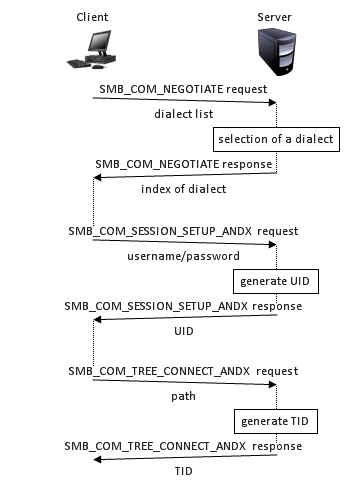
\includegraphics{login.png} \\
\vspace{6pt}
\textit{Typical message flow to perform a login.}
\end{center}

The first packet is sent by the client and contains a list of dialects, that the client understands. The server can choose one dialect of the list, that the server also understands, and sends the response to the client containing the index of the chosen dialect in the list. At this point, client and server have agreed on one dialect (often NT LM 0.12). The second step to perform a login is the validation of the username/password combination. The client sends its second packet to the server containing the username and the password. If the server accepts the username/password combination or grants guest accounts, it generates a User ID (UID) and sends the response to the client containing the generated UID. The last step of the login is the access to the desired path. The client sends its third packet to the server containing the path name in UNC format (i.e. $\backslash\backslash$SERVER$\backslash$SHARE). The server generates a Tree ID (TID) and grants access to the path, if the user has the appropriate rights. The user is now logged in and can continue with other operations like listing all files in the share or directly accessing a file.

\paragraph{File access}

\begin{center}
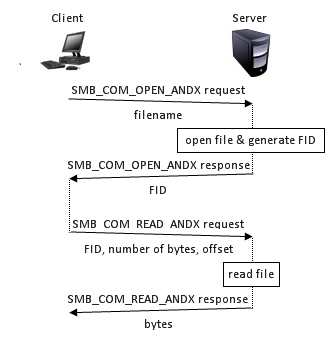
\includegraphics{fileaccess.png} \\
\vspace{6pt}
\textit{Typical message flow to read a file.}
\end{center}

Before the client can read or write a file, it has first to open the file. Therefore, the client sends a packet containing the filename. The server opens the file and generates a File ID (FID) used for further operations based on the opened file. The second packet of the client contains the FID, specifying the opened file, the number of bytes to read and the offset from where starting to read. The server sends a response containing the desired bytes.

\chapter{Implementation}
The implementation is subdivided in two modules. One module implements the client, the other module implements the server. The modules are independent from each other and can work simultaneously at the same machine.

\section{The Client Implementation}
In A2 every file system has to implement two interfaces. The first interface is the FileSystem interface, which handles operations on files, e.g. rename and delete. The second interface is the File interface, which handles operations on the content of files, e.g. read and write bytes. As shown in the figure below, applications operate directly on the two interfaces. While a classical file system like FAT operates on disks, a SMB file system operates through the network.

\begin{center}
\begin{tabular}{|c||c||c||c|}
\hline
\multicolumn{4}{|c|}{Applications} \\
\hline
\hline
File & FileSystem & File & FileSystem \\
\hline 
\hline
SambaFile & SambaFileSystem & FATFile & FATFileSystem \\
\hline
\hline
\multicolumn{2}{|c||}{TCP/IP} & \multicolumn{2}{|c|}{Disk} \\
\hline
\end{tabular} \\
\vspace{6pt}
\textit{The architecture of the Samba file system compared to the FAT file system.}
\end{center}

\subsection{The File System Interface}
The traditional Windows SMB client has one very important characteristic: it offers transparency. A user can manipulate files on a remote share, as if they were locally available. To improve transparency it is even possible to mount a remote share as a local file system. The A2 client implementation copies this characteristic by implementing the FileSystem interface offered by the operating system. The interface contains 9 procedures: \texttt{New0}, \texttt{Old0}, \texttt{Delete0}, \texttt{Rename0}, \texttt{Enumerate0}, \texttt{FileKey}, \texttt{CreateDirectory0}, \texttt{RemoveDirectory0} and \texttt{Finalize}.

\begin{center}
\renewcommand{\tabcolsep}{5mm}
\begin{tabular}{p{3cm}p{8cm}}
\texttt{New0} & \textbf{Creates a new file.} \\ 
\hline
\end{tabular}
\end{center}
To create a file on the server, the client first has to create a file object locally. The newly created file is associated to the SMB file system. Now, the client can proceed with the remote operations. Therefore the client sends a request to the server containing the command to create a new file. As response, the client recieves a file ID (FID), which is used as local ID too. This unique ID ensures, that the client as well as the server are operating on the correct file. \\
\renewcommand{\tabcolsep}{5mm}
\begin{tabular}{p{3cm}p{8cm}}
Packets needed: & \texttt{SMB\_COM\_OPEN\_ANDX} \\
\end{tabular}

\begin{center}
\renewcommand{\tabcolsep}{5mm}
\begin{tabular}{p{3cm}p{8cm}}
\texttt{Old0} & \textbf{Opens an existing file.} \\ 
\hline
\end{tabular}
\end{center}
To open a remote file, the client has to follow a similar procedure to \texttt{New0} and create a file object locally, even if the file exists on the server. The reason is that the client needs a file object to work. Then the client sends an open request and recieves a FID, which is needed for further operations on the file. \\
\renewcommand{\tabcolsep}{5mm}
\begin{tabular}{p{3cm}p{8cm}}
Packets needed: & \texttt{SMB\_COM\_OPEN\_ANDX} \\
\end{tabular}

\begin{center}
\renewcommand{\tabcolsep}{5mm}
\begin{tabular}{p{3cm}p{8cm}}
\texttt{Delete0} & \textbf{Deletes a file.} \\ 
\hline
\end{tabular}
\end{center}
If the client wants to delete a remote file, the file has to be closed. To delete the file, the client sends a delete request for the given filename. If no other clients have this file opened, i.e. have a lock on this file, the server can successfully delete the file.

This command cannot be executed always successfully, because A2 cannot explicitly close files. In general, the client opens a file at least once without closing it. A simple solution would maintain a list of open files and close the relative file before it is deleted. All applications having a reference to an open file would not be considered when closing the file. These references would become invalid. Client and server were in an inconsistent state. \\
\renewcommand{\tabcolsep}{5mm}
\begin{tabular}{p{3cm}p{8cm}}
Packets needed: & \texttt{SMB\_COM\_DELETE}, (\texttt{SMB\_COM\_CLOSE}) \\
\end{tabular}

\begin{center}
\renewcommand{\tabcolsep}{5mm}
\begin{tabular}{p{3cm}p{8cm}}
\texttt{Rename0} & \textbf{Renames a file.} \\ 
\hline
\end{tabular}
\end{center}
As in \texttt{Delete0}, if the client wants to rename a remote file, the file has to be closed. To rename the file, the client sends a rename request containing the old filename and the new filename. If no other clients have this file opened, i.e. have a lock on this file, the server can successfully rename the file.

This command cannot be executed always successfully, because A2 cannot explicitly close files. The problem is the same, as described in \texttt{Delete0}. \\
\renewcommand{\tabcolsep}{5mm}
\begin{tabular}{p{3cm}p{8cm}}
Packets needed: & \texttt{SMB\_COM\_RENAME}, (\texttt{SMB\_COM\_CLOSE}) \\
\end{tabular}

\begin{center}
\renewcommand{\tabcolsep}{5mm}
\begin{tabular}{p{3cm}p{8cm}}
\texttt{Enumerate0} & \textbf{Lists all files in a share.} \\ 
\hline
\end{tabular}
\end{center}
The client typically calls this procedure, if it needs to list all files present on the server in the File Manager. This procedure works with masks, which differ from the masks used in SMB. The client sends a listing request containing the appropriate mask, previously transformed by a simple helper procedure. If the list contained in the response is not complete, i.e. not all files of the share are listed, the client continues sending other requests containing the last entry and the ID of the search, until the list is complete. \\
\renewcommand{\tabcolsep}{5mm}
\begin{tabular}{p{3cm}p{8cm}}
Packets needed: & \texttt{TRANS2\_FIND\_FIRST2}, \texttt{TRANS2\_FIND\_NEXT2} \\
\end{tabular}

\begin{center}
\renewcommand{\tabcolsep}{5mm}
\begin{tabular}{p{3cm}p{8cm}}
\texttt{FileKey} & \textbf{Returns the unique non-zero key of the file.} \\ 
\hline
\end{tabular}
\end{center}
The FileKey procedure returns the unique non-zero key of a file. The key is generated by the server, when a file is opened (see \texttt{Old0}). If a file does not exist, the result is 0. \\
\renewcommand{\tabcolsep}{5mm}
\begin{tabular}{p{3cm}p{8cm}}
Packets needed: & \texttt{SMB\_COM\_OPEN\_ANDX} \\
\end{tabular}

\begin{center}
\renewcommand{\tabcolsep}{5mm}
\begin{tabular}{p{3cm}p{8cm}}
\texttt{CreateDirectory0} & \textbf{Creates a directory.} \\ 
\hline
\end{tabular}
\end{center}
A new directory is created by sending a create directory request with a pathname to the server. Unlike file creation, it is not necessary to create a directory locally first.

This command cannot be executed always successfully, because the AOS file system used in A2 does not support directories. A solution would be the integration of diretories in AOS file systems or the use of a FAT file system. \\
\renewcommand{\tabcolsep}{5mm}
\begin{tabular}{p{3cm}p{8cm}}
Packets needed: & \texttt{SMB\_COM\_CREATE\_DIRECTORY} \\
\end{tabular}

\begin{center}
\renewcommand{\tabcolsep}{5mm}
\begin{tabular}{p{3cm}p{8cm}}
\texttt{RemoveDirectory0} & \textbf{Deletes a directory.} \\ 
\hline
\end{tabular}
\end{center}
A directory can be deleted by sending a delete directory request to the server. The directory can only be deleted, if it does not contain files.

This command cannot be executed always successfully, because the AOS file system used in A2 does not support directories. The problem is the same, as described in \texttt{CreateDirectory0}. \\
\renewcommand{\tabcolsep}{5mm}
\begin{tabular}{p{3cm}p{8cm}}
Packets needed: & \texttt{SMB\_COM\_DELETE\_DIRECTORY} \\
\end{tabular}

\begin{center}
\renewcommand{\tabcolsep}{5mm}
\begin{tabular}{p{3cm}p{8cm}}
\texttt{Finalize} & \textbf{Finalizes the file system.} \\ 
\hline
\end{tabular}
\end{center}
This procedure closes the connection before unmounting the file system. \\
\renewcommand{\tabcolsep}{5mm}
\begin{tabular}{p{3cm}p{8cm}}
Packets needed: & \texttt{-} \\
\end{tabular}

\subsection{The File Interface}
The File Interface handles operations on the content of files. It is different from the File System Interface, which does not modify the content, but the properties of files. The interface contains 12 procedures: \texttt{Set}, \texttt{Pos}, \texttt{Read}, \texttt{ReadBytes}, \texttt{Write}, \texttt{WriteBytes}, \texttt{Length}, \texttt{GetDate}, \texttt{SetDate}, \texttt{GetName}, \texttt{Register0}, \texttt{Update}. The most important procedures, also largest in code size, are \texttt{ReadBytes} and \texttt{WriteBytes}.

\begin{center}
\renewcommand{\tabcolsep}{5mm}
\begin{tabular}{p{3cm}p{8cm}}
\texttt{ReadBytes} & \textbf{Reads a sequence of bytes.} \\ 
\hline
\end{tabular}
\end{center}
The client can read bytes of a file, if it was already opened. The request sent by the client must contain the file ID, the offset from where to start reading and the desired length of bytes. The response contains the requested bytes, which are buffered locally. The client also has to adjust the offset of the Rider. Too large requests (more than 65'535 bytes) are splitted up in multiple requests. \\
\renewcommand{\tabcolsep}{5mm}
\begin{tabular}{p{3cm}p{8cm}}
Packets needed: & \texttt{SMB\_COM\_READ\_ANDX} \\
\end{tabular}

\begin{center}
\renewcommand{\tabcolsep}{5mm}
\begin{tabular}{p{3cm}p{8cm}}
\texttt{WriteBytes} & \textbf{Writes a sequence of bytes.} \\ 
\hline
\end{tabular}
\end{center}
As in \texttt{ReadBytes}, the file has to be open and the request must contain file ID, offset and length. The difference is, that the request also contains the bytes to be written remotely. \\
\renewcommand{\tabcolsep}{5mm}
\begin{tabular}{p{3cm}p{8cm}}
Packets needed: & \texttt{SMB\_COM\_WRITE\_ANDX} \\
\end{tabular} \\

For the sake of completeness the other procedures are just mentioned:

\begin{center}
\begin{tabular}{l|l}
Set & Positions the Rider at a certain offset in a file. \\
Pos & Returns the offset of a Rider positioned on a file. \\
Read & Reads one byte. \\
Write & Writes one byte. \\
Length & Returns the current length of a file. \\
GetDate & Returns date and time of the last modification. \\
SetDate & Sets the modification date and time. \\
GetName & Returns the canonical name of a file. \\
Register0 & Registers a file created with New0 in the directory. \\
Update & Flushes the changes made to a file from its buffers. \\
\end{tabular} \\
\vspace{6pt}
\textit{All procedures (except ReadBytes and WriteBytes) contained in the File Interface.}
\end{center}

\subsection{Connection}
The implemented File System and File interface are not enough to integrate a Samba File System in A2, because SMB is a network protocol and the files are not locally available. The client has to establish a reliable connection to the server. As seen in the introduction, the connection is based on TCP. This is realized by an object called TCPSender, which establishes a connection to a specified IP address and port and opens streams to read and write. Packets are created and sent directly in the implemented interfaces. Helper procedures preprocess incoming packets and in case of error take the appropriate steps.

\subsection{Mounting}
The mounting process starts directly when the client is opened. The new Samba file system recieves the prefix \texttt{SMB:} similar to the Windows drive letters. Then the client establishes a connection to the server and tries to log in. The log in step is the same as described in the introduction. At this point, the client is running and files can be accessed, if no error has occured so far.

To unmount the file system, the client has first to log off on the remote machine and close the connection. The prefix \texttt{SMB:} becomes invalid.

\subsection{Implemented SMB Packets}
The SMB protocol offers approximately 75 different commands, not including subcommands. Not all are necessary to implement the client. The list of needed commands can be determined by the functions required by the client, i.e. the equivalent commands to the procedures of the interfaces. A command of special interest is \texttt{SMB\_COM\_TRANSACTION2}, which carries one of potentially 17 different subcommands. The client can send only 2 of them needed for the directory listing.

\begin{center}
\begin{tabular}{c|l}
Command & Description \\ 
\hline
0x00 & \texttt{SMB\_COM\_CREATE\_DIRECTORY} \\
0x01 & \texttt{SMB\_COM\_DELETE\_DIRECTORY} \\
0x04 & \texttt{SMB\_COM\_CLOSE} \\
0x06 & \texttt{SMB\_COM\_DELETE} \\
0x07 & \texttt{SMB\_COM\_RENAME} \\
0x08 & \texttt{SMB\_COM\_QUERY\_INFORMATION} \\
0x2D & \texttt{SMB\_COM\_OPEN\_ANDX} \\
0x2E & \texttt{SMB\_COM\_READ\_ANDX} \\
0x2F & \texttt{SMB\_COM\_WRITE\_ANDX} \\
0x32 & \texttt{SMB\_COM\_TRANSACTION2} \\
0x72 & \texttt{SMB\_COM\_NEGOTIATE} \\
0x73 & \texttt{SMB\_COM\_SESSION\_SETUP\_ANDX} \\
0x75 & \texttt{SMB\_COM\_TREE\_CONNECT\_ANDX} \\
\end{tabular} \\
\vspace{6pt}
\textit{All commands implemented by the client.}
\end{center}

\section{The Server Implementation}
The server works in a different way as the client. While the client can send requests if required, the server can only send responses when it recieves a request. An efficient server therefore has to understand all requests a client might send. The list of commands to implement was determined through a network protocol analyzer using a Windows XP client and the client provided by Ubuntu 8.10.

\subsection{Request Handling}
The running server listens on port 445 (defined port for raw SMB) for incoming connections. The port listener is implemented using an Agent of module TCPServices. If a client tries to connect to the server, the listener accepts the connection, reads the recieved packet and passes it to the dispatcher. The dispatcher interprets the command and passes the packet to the appropriate handler, which starts to evaluate the information contained in the packet and performs the requested operation. Then the handler generates a response for the client. Since the server is in an endless loop, it can accept the next packet and the cycle restarts.
\begin{center}
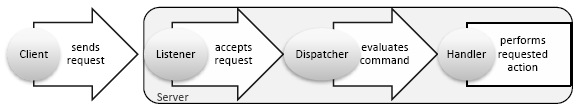
\includegraphics[width=13cm]{server.png} \\
\vspace{6pt}
\textit{The server steps.}
\end{center}

\subsection{Implemented SMB Packets}

\begin{center}
\renewcommand{\tabcolsep}{5mm}
\begin{tabular}{p{3cm}p{8cm}}
0x00 & \texttt{SMB\_COM\_CREATE\_DIRECTORY} \\ 
\hline
\end{tabular}
\end{center}
The create directory message is sent to create a new directory. The additional pathname is passed. The directory must not exist for it to be created.

This command cannot be executed always successfully, because the AOS file system used in A2 does not support directories.

\begin{center}
\renewcommand{\tabcolsep}{5mm}
\begin{tabular}{p{3cm}p{8cm}}
0x01 & \texttt{SMB\_COM\_DELETE\_DIRECTORY} \\ 
\hline
\end{tabular}
\end{center}
The delete directory message is sent to delete an empty directory. The additional pathname is passed. The directory has to be empty for it to be deleted.

This command cannot be executed always successfully, because the AOS file system used in A2 does not support directories.

\begin{center}
\renewcommand{\tabcolsep}{5mm}
\begin{tabular}{p{3cm}p{8cm}}
0x02 & \texttt{SMB\_COM\_OPEN} \\ 
\hline
\end{tabular}
\end{center}
This message is sent to obtain a file handle for a data file. It is the predecessor of the \texttt{SMB\_COM\_OPEN\_ANDX} packet.

This command was implemented to handle pipe requests, but became obsolete since Windows clients prefer the newer \texttt{SMB\_COM\_OPEN\_ANDX} packet.

\begin{center}
\renewcommand{\tabcolsep}{5mm}
\begin{tabular}{p{3cm}p{8cm}}
0x04 & \texttt{SMB\_COM\_CLOSE} \\
\hline
\end{tabular}
\end{center}
The close message is sent to invalidate a file handle for the requesting client. All locks held by the client on the file should be released by the server. The client can no longer use the FID for further file access.

This command has no effect, because files cannot be closed in A2.

\begin{center}
\renewcommand{\tabcolsep}{5mm}
\begin{tabular}{p{3cm}p{8cm}}
0x05 & \texttt{SMB\_COM\_FLUSH} \\
\hline
\end{tabular}
\end{center}
The flush message is sent to ensure all data for the corresponding file has been written to stable storage.

This command has no effect, because all bytes received by previous write commands are directly written to disk.

\begin{center}
\renewcommand{\tabcolsep}{5mm}
\begin{tabular}{p{3cm}p{8cm}}
0x06 & \texttt{SMB\_COM\_DELETE} \\
\hline
\end{tabular}
\end{center}
The delete message is sent to delete a file. The additional filename is passed.

Deleting multiple files using wildcards and SearchAttributes are not supported by the server and are ignored.

\begin{center}
\renewcommand{\tabcolsep}{5mm}
\begin{tabular}{p{3cm}p{8cm}}
0x07 & \texttt{SMB\_COM\_RENAME} \\
\hline
\end{tabular}
\end{center}
The rename message is sent to change the name of a file. The old and new filenames are passed.

Renaming multiple files using wildcards and SearchAttributes are not supported by the server and are ignored.

\begin{center}
\renewcommand{\tabcolsep}{5mm}
\begin{tabular}{p{3cm}p{8cm}}
0x08 & \texttt{SMB\_COM\_QUERY\_INFORMATION} \\
\hline
\end{tabular}
\end{center}
The query information message is sent to obtain the properties of a file, e.g. last write time and file size. Attributes are not implemented and therefore ignored.

\begin{center}
\renewcommand{\tabcolsep}{5mm}
\begin{tabular}{p{3cm}p{8cm}}
0x09 & \texttt{SMB\_COM\_SET\_INFORMATION} \\
\hline
\end{tabular}
\end{center}
The set information message is sent to change the properties of a file, e.g. last write time and file size. The support of attributes is optional, therefore not implemented and ignored.

\begin{center}
\renewcommand{\tabcolsep}{5mm}
\begin{tabular}{p{3cm}p{8cm}}
0x0B & \texttt{SMB\_COM\_WRITE} \\
\hline
\end{tabular}
\end{center}
The write message is sent to write bytes to a file. The additional file ID, the offset specifying form where to start, the length of bytes and the data itself are passed. If the length is zero and no data is passed, the server must truncate the file to the length specified in the offset field.

\begin{center}
\renewcommand{\tabcolsep}{5mm}
\begin{tabular}{p{3cm}p{8cm}}
0x0F & \texttt{SMB\_COM\_CREATE\_NEW} \\
\hline
\end{tabular}
\end{center}
The create new message is sent to create a new non-existing file or to truncate an existing file to zero. Truncating is implemented as deleting the file and creating a new one with same properties.

\begin{center}
\renewcommand{\tabcolsep}{5mm}
\begin{tabular}{p{3cm}p{8cm}}
0x22 & \texttt{SMB\_COM\_SET\_INFORMATION2} \\
\hline
\end{tabular}
\end{center}
This set information message is similar to \texttt{SMB\_COM\_SET\_INFORMATION}. The main difference is, that the file is defined by its FID (previously opened) and not by its filename.

\begin{center}
\renewcommand{\tabcolsep}{5mm}
\begin{tabular}{p{3cm}p{8cm}}
0x23 & \texttt{SMB\_COM\_QUERY\_INFORMATION2} \\
\hline
\end{tabular}
\end{center}
This query information message is similar to \texttt{SMB\_COM\_QUERY\_INFORMATION}. The main difference is, that the file is defined by its FID (previously opened) and not by its filename.

\begin{flushleft}
\begin{center}
\renewcommand{\tabcolsep}{5mm}
\begin{tabular}{p{3cm}p{8cm}}
0x25 & \texttt{SMB\_COM\_TRANSACTION} \\
\hline
\end{tabular}
\end{center}
The transaction message is sent to pass pipe or LANMAN information. The server accepts this packets, but does not perform any operation. If the server would not accept this command, a client running on Windows would probably not establish a connection.
\end{flushleft}

\begin{center}
\renewcommand{\tabcolsep}{5mm}
\begin{tabular}{p{3cm}p{8cm}}
0x2B & \texttt{SMB\_COM\_ECHO} \\
\hline
\end{tabular}
\end{center}
The echo message is sent to test the connection to the server and to check that the server works. The server echoes the data recieved in the request.

\begin{center}
\renewcommand{\tabcolsep}{5mm}
\begin{tabular}{p{3cm}p{8cm}}
0x2D & \texttt{SMB\_COM\_OPEN\_ANDX} \\
\hline
\end{tabular}
\end{center}
The open andx message is sent to open an existing file or to create a new non-existing file. The action depends on a field. The additional filename is passed. A file can be opened in two access modes: for reading or for writing. Both modes are mutually exclusive. The server ignores the access mode, because A2 does not distinguish between the two modes.

\begin{center}
\renewcommand{\tabcolsep}{5mm}
\begin{tabular}{p{3cm}p{8cm}}
0x2E & \texttt{SMB\_COM\_READ\_ANDX} \\
\hline
\end{tabular}
\end{center}
The read andx message is sent to read bytes of a file. The additional file ID, the offset specifying form where to start and the length of bytes are passed. 

\begin{center}
\renewcommand{\tabcolsep}{5mm}
\begin{tabular}{p{3cm}p{8cm}}
0x2F & \texttt{SMB\_COM\_WRITE\_ANDX} \\
\hline
\end{tabular}
\end{center}
The write andx message is similar to \texttt{SMB\_COM\_WRITE}, except for the truncation, which is not supported here.

\begin{flushleft}
\begin{center}
\renewcommand{\tabcolsep}{5mm}
\begin{tabular}{p{3cm}p{8cm}}
0x32 & \texttt{SMB\_COM\_TRANSACTION2} \\
\hline
\end{tabular}
\end{center}
The transaction message is sent to obtain information. This packet can carry 17 different subcommands, but only 5 are implemented.
\begin{itemize}
\item \texttt{FIND\_FIRST2} used to start a search (file listing).
\item \texttt{FIND\_NEXT2} used to continue a search.
\item \texttt{QUERY\_FS\_INFORMATION} used to get information of the remote file system.
\item \texttt{QUERY\_PATH\_INFORMATION} used to get information of a directory.
\item \texttt{QUERY\_FILE\_INFORMATION} used to get information of a file.
\end{itemize}
\end{flushleft}

\begin{center}
\renewcommand{\tabcolsep}{5mm}
\begin{tabular}{p{3cm}p{8cm}}
0x34 & \texttt{SMB\_COM\_FIND\_CLOSE2} \\
\hline
\end{tabular}
\end{center}
The find close message is sent to close a search started by a \texttt{TRANS2\_FIND\_FIRST2} request. The additional search ID is passed.

\begin{center}
\renewcommand{\tabcolsep}{5mm}
\begin{tabular}{p{3cm}p{8cm}}
0x71 & \texttt{SMB\_COM\_TREE\_DISCONNECT} \\
\hline
\end{tabular}
\end{center}
The tree disconnect message is sent to invalidate a share handle for the requesting client. The client can no longer use the TID for further access.

\begin{center}
\renewcommand{\tabcolsep}{5mm}
\begin{tabular}{p{3cm}p{8cm}}
0x72 & \texttt{SMB\_COM\_NEGOTIATE} \\
\hline
\end{tabular}
\end{center}
The negotiate message is sent to agree on a dialect. This is the first packet sent by the client to establish a connection. This message contains a list of dialect, that the client understands. The response contains information about the server, e.g. server time, server name.

\begin{center}
\renewcommand{\tabcolsep}{5mm}
\begin{tabular}{p{3cm}p{8cm}}
0x73 & \texttt{SMB\_COM\_SESSION\_SETUP\_ANDX} \\
\hline
\end{tabular}
\end{center}
The session setup message is sent to log in. This is the second packet sent by the client. This message contains username and password. If the server accepts the combination of username and password or accepts guest login, the client is logged in.

\begin{center}
\renewcommand{\tabcolsep}{5mm}
\begin{tabular}{p{3cm}p{8cm}}
0x75 & \texttt{SMB\_COM\_TREE\_CONNECT\_ANDX} \\
\hline
\end{tabular}
\end{center}
The tree connect message is sent to connect to a share. The additional pathname following the UNC style syntax (e.g. $\backslash\backslash$SERVER$\backslash$SHARE) is passed.

The new Samba documentation released by Microsoft reveals two important fields: MaximalShareAccessRights and GuestMaximalShareAccessRights specify the respective rights on a share. These fields were probably unknown in the old server implementation for Bluebottle and therefore Windows clients refused the connection.

\begin{center}
\renewcommand{\tabcolsep}{5mm}
\begin{tabular}{p{3cm}p{8cm}}
0xA0 & \texttt{SMB\_COM\_NT\_TRANSACT} \\
\hline
\end{tabular}
\end{center}
The transact message is sent to transfer file system control functions. The server accepts this packets, but does not perform any operation. If the server would not accept this command, a client running on Windows would probably not establish a connection.

\section{Time in Samba}
In Samba time values can be encoded in three different modes. A2 does not use any of these modes. But, the server as well as the client provide specific conversion procedures.
\begin{itemize}
\item \texttt{SMB\_TIME \& SMB\_DATE} \\ Time base: 01-01-1980, 00:00:00 \\ Size: 4 bytes \\ Composition:
\begin{center}
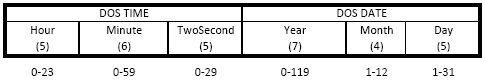
\includegraphics[width=10cm]{dostime.png} \\
\vspace{6pt}
\textit{Composition of DOS Time and DOS Date with number of used bits in brackets and range value below.}
\end{center}

\item \texttt{TIME} \\ Time base: 01-01-1601, 00:00:00 \\ Size: 8 bytes \\ Composition: Time passed in 100ns since time base.

\item \texttt{UTIME} \\ Time base: 01-01-1970, 00:00:00 \\ Size: 4 bytes \\ Composition: Time passed in seconds since time base.
\end{itemize}

\chapter{Evaluation}

\section{Benchmark}

\begin{center}
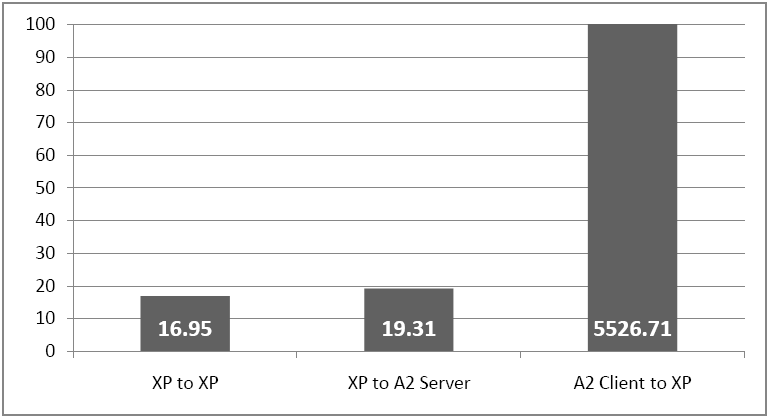
\includegraphics[width=10cm]{1x100mb.png} \\
\vspace{6pt}
\textit{Seconds elapsed to transfer 1x 100MB-file.}
\end{center}

The time for the transfer of one 100MB file from a Windows XP machine to another Windows XP machine is taken as a reference point. The transfer from a Windows XP client to the A2 server needed 19.31s, which is close to the Windows reference value. The most surprising value is the transfer from the A2 client to a Windows XP server. This mode is definitely the slowest. The main reason for this weak performance is unclear. One point is, that the Windows XP client sends 32kB data per packet, but the A2 client only sends 4kB data per packet. 

\begin{center}
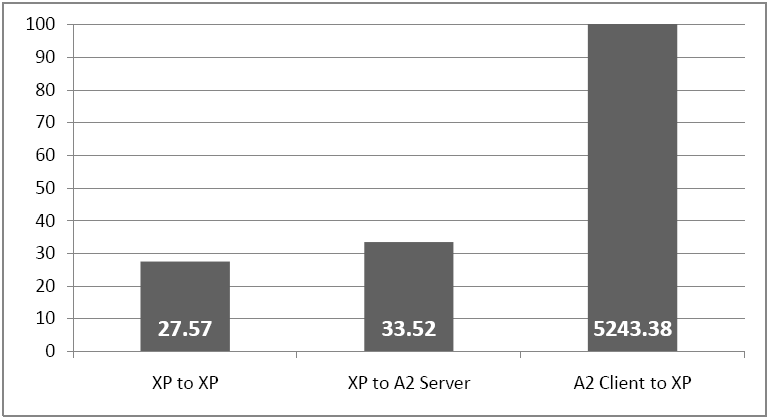
\includegraphics[width=10cm]{1000x100kb.png} \\
\vspace{6pt}
\textit{Seconds elapsed to transfer 1000x 100kB-files.}
\end{center}

Also for this benchmark the Windows XP to Windows XP value is taken as a reference point. The Windows XP client to the A2 server transfer of 1000 100kB files performs well compared to the reference value. As with one file, the A2 client to Windows XP server is again the slowest mode. The reasons may be the same as with one file, but no anomalities were detected in both cases.

\chapter{Conclusion \& Future Work}

\section{Conclusion}
This master thesis provides a client and server implementation of Samba, the de facto standard for file access in Local Area Networks, for A2. The goal, to simplify data access and to increase the interoperability between A2 and other operating systems, especially Windows, is reached. The old server implementation for Bluebottle probably did not work, because two fields of \texttt{SMB\_COM\_TREE\_CONNECT\_ANDX} response, revealed by Microsoft in 2007, were not considered.

The procedures-to-packets mapping of the client is complete. All procedures are implemented equivalently in Samba packets. The server definitely does not implement all existing commands, but understands all encountered by sniffing the network using Windows and Linux clients.

\subsection{Problems}
A yet unsolved problem was caused by \texttt{SMB\_COM\_CLOSE} (closes a file). A2 does not provide a \texttt{File.Close}. Therefore, files are kept open, as long as the client is running. This impedes the client to rename or delete already opened files. Various solutions like keeping a list of open files or immediatly closing the file failed. A solution would be the implementation of a close procedure in A2.

\section{Future Work}
\begin{itemize}
\item \textbf{Challenge/Response Authentication} \\ The current implementation of the login only provides plaintext passwords and guest access. This solution might be enough in a secure environment, but is risky otherwise. Implementing the challenge/response authentication improves the security.
\item \textbf{Printer access} \\ The printer access is part of Samba and allows a client to print on a connected server. The implementation requires DCE/RPC, but also uses packets for file access like \texttt{SMB\_COM\_WRITE\_ANDX}.
\item \textbf{SMB2} \\ This protocol was introduced with Windows Vista. The implementation of SMB2 is less important than the two points before, but offers the possibility to perform multiple actions with a single request. The increased buffer sizes allow the transport of more data in a packet. These are two important improvments when operating with large files.
\end{itemize}

\appendix

\chapter{Samba in Detail}

\section{Header}
\begin{center}
	\renewcommand{\tabcolsep}{3mm}
	\begin{tabular}{lcrlcrlcrlcr}
		0 & \ldots & 7 & 8 & \ldots & 15 & 16 & \ldots & 23 & 24 & \ldots & 31 \\
		\hline
		\multicolumn{3}{|c|}{0xFF} &
		\multicolumn{3}{|c|}{'S'} &
		\multicolumn{3}{|c|}{'M'} &
		\multicolumn{3}{|c|}{'B'} \\
		\hline
		\multicolumn{3}{|c|}{COMMAND} &
		\multicolumn{9}{|c|}{STATUS\ldots} \\
		\hline
		\multicolumn{3}{|c|}{\ldots STATUS} &
		\multicolumn{3}{|c|}{FLAGS} &
		\multicolumn{6}{|c|}{FLAGS2} \\
		\hline
		\multicolumn{12}{|c|}{EXTRA} \\
		\multicolumn{12}{|c|}{\ldots} \\
		\multicolumn{12}{|c|}{\ldots} \\
		\hline
		\multicolumn{6}{|c|}{TID} &
		\multicolumn{6}{|c|}{PID} \\
		\hline
		\multicolumn{6}{|c|}{UID} &
		\multicolumn{6}{|c|}{MID} \\
		\hline
	\end{tabular}
\end{center}

\paragraph{0xFF SMB} The first 4 bytes are the protocol identifier string, which are always the same: 0xFF and the ASCII representation of the letters 'S', 'M' and 'B'.

\paragraph{Command} The one-byte command field tells the type of the SMB.

\paragraph{Status} Two versions of error reporting exist: 16-bit DOS error code and 32-bit NT status code. The DOS error code is grouped in two classes \textit{ErrorClass} (1 byte) and \textit{ErrorCode} (2 bytes) separated by a 8-bit reserved block. The NT status code, introduced with Windows NT, uses the entire field to contain the \textit{NT Status} (4 bytes). The error reporting version is determined at beginning by a Flags2 bit. Regardless of the version, if the fields are zero, they indicate success.

\paragraph{Flags} The Flags field contains 8 different flags numbered here from least significant to most significant bit.
\begin{center}
	\begin{tabular}{r|l}
		Bit & Description \\ 
		\hline
		0 & Lock \& Read and Write \& Unlock \\
		1 & Recieve Buffer Posted \\
		2 & Reserved \\	
		3 & Case Sensitivity \\
		4 & Canonicalized Pathnames \\
		5 & Oplocks \\
		6 & Notify \\
		7 & Request/Response \\
	\end{tabular}
\end{center}
The implementation takes only bits 3,4 and 7 into consideration. The other bits are simply ignored, which does not cause any side-effect. Flags which are not used must be 0 and flags which are not set must be ignored.

\paragraph{Flags2} The Flags2 field contains 9 different flags numbered here form least significant to most significant bit.
\begin{center}
	\begin{tabular}{r|l}
		Bit & Description \\ 
		\hline
		0 & Long Names Allowed \\
		1 & Extended Attributes \\
		2 & Security Signatures \\
		6 & Long Names Used \\
		11 & Extended Security Negotiation \\
		12 & DFS Resolution \\
		13 & Execute-only Reads \\
		14 & Error Code Type \\
		15 & Unicode Strings \\
	\end{tabular}
\end{center}
All bits which are not listed in the table above must be 0 and therefore ignored. The implementation takes only bit 0 into consideration. The other bits are simply ignored as in Flags, which does not cause any side-effect.

\paragraph{Extra} The Extra field is splitted in three fields: Process ID High (2 bytes), Signature (8 bytes) and Reserved (2 bytes). The Process ID High field can be used to support 32-bit process IDs. The implementation uses only 16-bit process IDs which is enough. The field is 0 and can be ignored. The Signature field can be used to sign the SMB but is not used by the implementation. The Reserved field must be 0 and is therefore useless.

\paragraph{TID} The Tree ID identifies the client connection to a specific share. The server returns a TID to the client when the client successfully connects to a server ressource. For any subsequent requests the client uses the TID.

\paragraph{PID} The Process ID identifies the client process and is mainly used to control concurrency. The PID is initially set by the client. The server should not change the value.

\paragraph{UID} The User ID identifies a successfully authenticated user (username/ password). The UID is assigned by the server. For any subsequent requests the client uses the UID. The UID is only valid for the given session.

\paragraph{MID} The Multiplex ID identifies multiple outstanding requests. The server must not answer in a specific order but a response must contain the same MID and PID as in the corresponding request.

\section{Case in Point: \texttt{NEGOTIATE PROTOCOL}}
The first packet a client sends to a server to establish a connection is a Negotiate Protocol Request.
\begin{verbatim}
NEGOTIATE_PROTOCOL_REQUEST
  {
  SMB_HEADER
    {
    PROTOCOL  = 0xFF SMB
    COMMAND   = SMB_COM_NEGOTIATE (0x72)
    STATUS
      {
      ErrorClass = 0x00   (Success)
      ErrorCode  = 0x0000 (No Error)
      }
    FLAGS     = 0x18   (Canonicalized and case-sensitive path names)
    FLAGS2    = 0x0001 (Long file names allowed)
    EXTRA
      {
      PidHigh   = 0x0000
      Signature = 0 (8 bytes)
      }
    TID       = 0    (still unknown)
    PID       = 9876 (defined by client)
    UID       = 0    (still unknown)
    MID       = 0    (no pending responses)
    }
  SMB_PARAMETERS
    {
    WordCount = 0
    Words     = (empty)
    }
  SMB_DATA
    {
    ByteCount = 12
    Bytes
      {
      BufferFormat = 0x02         (Dialect)
      Name         = "NT LM 0.12" (0x00 terminated)
      }
    }
  }
\end{verbatim}

\section{File System Interface}

\begin{verbatim}
(** Create a new file with the specified name. *)
PROCEDURE New0*(name: ARRAY OF CHAR): File;
		
(** Open an existing file. The same file descriptor is returned
    if a file is opened multiple times. *)
PROCEDURE Old0*(name: ARRAY OF CHAR): File;

(** Delete a file. res = 0 indicates success. *)
PROCEDURE Delete0*(name: ARRAY OF CHAR; VAR key, res: LONGINT);
		
(** Rename a file. res = 0 indicates success. *)
PROCEDURE Rename0*
    (old, new: ARRAY OF CHAR; f: File; VAR res: LONGINT);
		
(** Enumerate canonical file names. mask may contain * wildcards.
    For internal use only. *)
PROCEDURE Enumerate0*
    (mask: ARRAY OF CHAR; flags: SET; enum: Enumerator);

(** Return the unique non-zero key of the named file, if it
    exists. *)		
PROCEDURE FileKey*(name: ARRAY OF CHAR): LONGINT;
		
(** Create a new directory structure. May not be supported by
    the actual implementation. *)
PROCEDURE CreateDirectory0*(name: ARRAY OF CHAR; VAR res: LONGINT);
	
(** Remove a directory. If force=TRUE, any subdirectories and
    files should be automatically deleted. *)
PROCEDURE RemoveDirectory0*
    (name: ARRAY OF CHAR; force: BOOLEAN; VAR key, res: LONGINT);
		
(** Finalize the file system. *)
PROCEDURE Finalize*;
\end{verbatim}

\section{File Interface}

\begin{verbatim}
(** Position a Rider at a certain position in a file. Multiple
    Riders can be positioned at different locations in a file.
    A Rider cannot be positioned beyond the end of a file. *)		
PROCEDURE Set*(VAR r: Rider; pos: LONGINT);

(** Return the offset of a Rider positioned on a file. *)
PROCEDURE Pos*(VAR r: Rider): LONGINT;

(** Read a byte from a file, advancing the Rider one byte
    further.  R.eof indicates if the end of the file has been
    passed. *)
PROCEDURE Read*(VAR r: Rider; VAR x: CHAR);

(** Read a sequence of len bytes into the buffer x at offset
    ofs, advancing the Rider. Less bytes will be read when
    reading over the end of the file. r.res indicates the
    number of unread bytes. x must be big enough to hold all
    the bytes. *)
PROCEDURE ReadBytes*
    (VAR r: Rider; VAR x: ARRAY OF CHAR; ofs, len: LONGINT);

(** Write a byte into the file at the Rider position,
    advancing the Rider by one. *)
PROCEDURE Write*(VAR r: Rider; x: CHAR);

(** Write the buffer x containing len bytes (starting at 
    offset ofs) into a file at the Rider position. *)
PROCEDURE WriteBytes*
    (VAR r: Rider; CONST x: ARRAY OF CHAR; ofs, len: LONGINT);

(** Return the current length of a file. *)
PROCEDURE Length*(): LONGINT;

(** Return the time (t) and date (d) when a file was last
    modified. *)
PROCEDURE GetDate*(VAR t, d: LONGINT);

(** Set the modification time (t) and date (d) of a file. *)
PROCEDURE SetDate*(t, d: LONGINT);

(** Return the canonical name of a file. *)
PROCEDURE GetName*(VAR name: ARRAY OF CHAR);

(** Register a file created with New in the directory,
    replacing the previous file in the directory with the
    same name. The file is automatically updated. *)
PROCEDURE Register0*(VAR res: LONGINT);

(** Flush the changes made to a file from its buffers. 
    Register0 will automatically update a file. *) 
PROCEDURE Update*;
\end{verbatim}

\begin{thebibliography}{LeachNaik}
\bibitem{Bihr} BIHR, Marcel: \textit{SambaServer - A CIFS 1.0 Implementation for Bluebottle}, Semester Thesis, ETH Zurich, 2006.
\bibitem{Hertel} HERTEL, Christopher R.: \textit{Implementing CIFS - The Common Internet File System}, Prentice Hall, 2003.
\bibitem{LeachNaik} LEACH, Paul J., NAIK, Dilip C.: \textit{A Common Internet File System (CIFS/1.0) Protocol - Preliminary Draft}, \texttt{http://www.microsoft.com/about/legal/protocols/BSTD/\\CIFS/draft-leach-cifs-v1-spec-02.txt}, 1997.
\bibitem{Microsoft} Microsoft Corporation: \textit{[MS-SMB] - Server Message Block (SMB) Protocol Specification}, \texttt{http://msdn.microsoft.com/en-us/library/cc246231.aspx}, 2007-2009.
\bibitem{CIFS} Storage Networking Industry Association (SNIA): \textit{Common Internet File System (CIFS) Technical Reference}, \texttt{http://www.snia.org/tech\_activities/CIFS/\\CIFS-TR-1p00\_FINAL.pdf}, 2002.
 
\end{thebibliography}


\end{document}